\documentclass[9pt,xcolor=pdftex,dvipsnames,table]{beamer} 
\setbeamercolor{bgcolor}{fg=white,bg=blue!100}
\mode<presentation>
{
  \usetheme{Darmstadt}
 \setbeamertemplate{navigation symbols}{}
  \setbeamercovered{transparent}
  \setbeamertemplate{footline}
{\rightline{\insertframenumber/\inserttotalframenumber}}
}

\def\newblock{}

\newenvironment{changemargin}[2]{% 
  \begin{list}{}{% 
    \setlength{\topsep}{0pt}% 
    \setlength{\leftmargin}{#1}% 
    \setlength{\rightmargin}{#2}% 
    \setlength{\listparindent}{\parindent}% 
    \setlength{\itemindent}{\parindent}% 
    \setlength{\parsep}{\parskip}% 
  }% 
  \item[]}{\end{list}} 
  
\usepackage[english]{babel}
\usepackage{amsmath}
\usepackage{lipsum}
\usepackage[latin1]{inputenc}
\usepackage{times}
\usepackage[latin1]{inputenc}
\usepackage{tipa}
\usepackage{color}
\usepackage{booktabs}
\usepackage{qtree}

\newcommand\mylex[2]{\advance\nbranches by1
\leaf{\emph{#2}}\branch{1}{\bf #1}}

\usepackage{colortbl}
\usepackage{movie15}
\usepackage{gb4e}
\usepackage{longtable}
\usepackage{pgf,pgfarrows,pgfnodes}
\usepackage{tikz} 
\usepackage{textpos}            % free image positioning 
\setlength{\TPVertModule}{1cm}  % unit for vertical positioning 
\setlength{\TPHorizModule}{1cm} % unit for horizontal positioning 

\definecolor{lightorange}{rgb}{1,0.75,.25}
\definecolor{lightred}{rgb}{1,0.25,.25}
\definecolor{lightblue}{rgb}{.25,.25,1.0}
\definecolor{lightgray}{rgb}{.75,.75,.75}

\usepackage[T1]{fontenc}

\title{Context Free Grammars (\& English)}
\author{Linguistics 409 $\cdot$ Computational Linguistics}
\date{}
\usepackage{gb4e}

\usepackage{natbib}
\bibliographystyle{apalike}

\makeatletter
\newcommand\textsubscript[1]{\@textsubscript{\selectfont#1}}
\def\@textsubscript#1{{\m@th\ensuremath{_{\mbox{\fontsize\sf@size\z@#1}}}}}
\newcommand\textbothscript[2]{%
  \@textbothscript{\selectfont#1}{\selectfont#2}}
\def\@textbothscript#1#2{%
  {\m@th\ensuremath{%
    ^{\mbox{\fontsize\sf@size\z@#1}}%
    _{\mbox{\fontsize\sf@size\z@#2}}}}}
\def\@super{^}\def\@sub{_}
\makeatother

\begin{document}
\definecolor{grey}{rgb}{1,0.6,.7}

\section{Introduction}

\begin{frame}

	\titlepage
	\vspace{-1.5cm}
	\begin{center}
    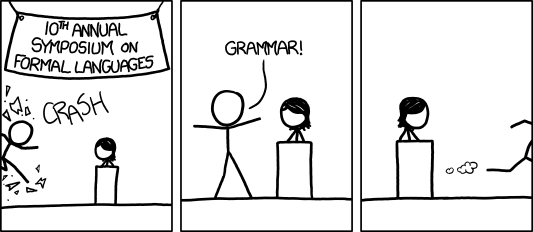
\includegraphics[scale=.5]{XKCDformalLanguages.png}\\
    
    { alt-text: [audience looks around] `What just happened?'\\`There must be some context we're missing.'}
	\end{center}
	
\end{frame}


\section{Constituency}

\begin{frame}{Sentences have syntactic structure.}
\begin{center}
{\huge were few hardest journey minutes of probe's the the the last }
\end{center}
\end{frame}


\begin{frame}{}
\begin{center}
{\huge man dog the the bit }
\end{center}
\end{frame}

\begin{frame}{arf!}
\begin{columns}[c] % contents are top vertically aligned
     \begin{column}[]{5.0cm} % alternative top-align that's better for graphics
              \Tree [[ the dog ] [ bit [ the man ] ] ]
     \end{column}
     \begin{column}[]{5cm} % alternative top-align that's better for graphics
              \Tree [[ the man ] [ bit [ the dog ] ] ]
     \end{column}
\end{columns}
\end{frame}

\begin{frame}{Parse}
\begin{center}
{\huge Buy more local produce. }
\end{center}
\end{frame}


\begin{frame}{Parse}
\begin{center}{\large Buy more {\huge \textbf{local produce}}. }\end{center}
\begin{center}{\large Buy {\huge \textbf{more local}} produce. }\end{center}
\end{frame}

\begin{frame}{produce produce}
\begin{columns}[c] % contents are top vertically aligned
     \begin{column}[]{5.0cm} % alternative top-align that's better for graphics
                   \Tree [ more [ local produce ]]
                   \begin{center}``more produce that is locally grown''\end{center}
     \end{column}
     \begin{column}[]{5cm} % alternative top-align that's better for graphics
                            \Tree [[ more local ] produce ]
                           \begin{center} ``produce that is grown closer to here''\end{center}
    \end{column}
\end{columns}
\end{frame}

\begin{frame}{Constituency}
\begin{center}Buy more local produce\end{center}
\begin{itemize}
     \item What matters for meaning is how \emph{closely related} the words in this sentence are.
     \item Words that function together are called a \textbf{constituent}.
     \item We have a number of tests for constituency (some better than others)
\end{itemize}
\end{frame}

\begin{frame}{Tests for constituency}
\begin{center} constituent is \emph{always} a contiguous string of words. \end{center}
\begin{itemize}
     \item No skipping words in a constituent.
     \item Syntactic operations can only be performed on constituents.
     \item This means we can use these same `syntactic operations' to identify constituents.
\end{itemize}
\end{frame}

\begin{frame}{Tests for constituency}
\begin{enumerate}
     \item Stand Alone Test
     \item Substitution
     \item Movement
     \item Coordination
\end{enumerate}
\end{frame}

\begin{frame}{Tests for constituency: Stand Alone Test}
\begin{center}
     {\large A constituent can often stand alone as the answer to a question. }
\end{center}
\begin{itemize}
     \item What can stand alone as the answer to a question?\pause
     \item What can a constituent do? \pause
     \item Stand alone as the answer to what?
\end{itemize}
\end{frame}

\begin{frame}{Tests for constituency:Substitution}
\begin{center}
     {\large A constituent can often be replaced by a single word.}
\end{center}
\begin{itemize}
     \item \emph{They} can often be replaced by a single word. \pause
     \item A constituent \emph{does}. \pause
     \item A constituent can often be replaced by \emph{one}.
\end{itemize}
\end{frame}

\begin{frame}{Tests for constituency: Movement}
\begin{center}
     {\large Constituents can sometimes be moved as units to change emphasis (but not meaning). }
\end{center}
\begin{itemize}
     \item To change emphasis, constituents can sometimes be moved as units.
     \item As units, constituents can sometimes be moved to change emphasis.
     \item Sometimes, constituents can be moved to change emphasis.
     \item It is constituents that can sometimes be moved as units to change emphasis.
\end{itemize}
\end{frame}

\begin{frame}{Tests for constituency: Coordination}
\begin{center}
     {\large The coordinating conjunctions \emph{and} and \emph{or} must conjoin equal units.  This means you can try balancing a unit you think is a constituent with something you know already to be a constituent. Try using \emph{yelled} to test these potential constituents: }
\end{center}
\begin{itemize}
     \item The meerkats \emph{invaded enemy territory}. \pause
     \item The referee \emph{called back the goal again}. \pause
     \item Every man \emph{kills the thing he loves}.
\end{itemize}
\end{frame}

\begin{frame}{Tests for constituency: Are these constituents?}
\begin{itemize}
     \item Pam saw \underline{the boy} with \underline{a telescope}
     \item \underline{Johan's head feels} better.
     \item Chris \underline{stopped} all the \emph{shots easily}.
     \item She said ``eh, \underline{I know you} and you cannot sing''.
     \item I said, ``that's nothing, \underline{you should hear me play piano}''. 
\end{itemize}
\end{frame}

\section{Context Free Grammar}

\subsection{}
\begin{frame}{}
    \setbeamercovered{invisible}

{\large We might notice that certain constituent types emerge in our testing. }
\vspace{.25cm}
	\begin{description}
		\item[Noun Phrases (aka NP)] can be subjects, can be objects, can be replaced by pronouns, can answer questions like `who?' or `I drank what?'
		\item[Verb Phrases (aka VP)] seem to assign \textbf{grammatical relations} to the noun phrases (a subject is the SUBJECT because of the verb, an object is the OBJECT because of the verb!), can be replaced by a single known-verb (e.g. \emph{yelled}), etc.
		\item[Prepositional Phrases] start with a preposition, always seems to contain an NP, seem to be attachable to Noun Phrases or Verb Phrases depending on meaning, etc.
		\item[Many others...]
	\end{description}
\end{frame}

\subsection{}
\begin{frame}{}
    \setbeamercovered{invisible}

{\large Two types of structure immediately emerge when we classify constituents into types...}
\vspace{.25cm}
	\begin{enumerate}
		\item These constituents or phrases have internal structure!
		\begin{quote}
		NP $\rightarrow$ Det Nominal\\
		NP $\rightarrow$ ProperNoun\\
		NP $\rightarrow$ Pronoun\\
		Nominal $\rightarrow$ Noun \textpipe{} Nominal Noun
		PP $\rightarrow$ Preposition NP
		\end{quote}
		\item And the constituents can only be combined in certain ways.
		\begin{quote}
		e.g. English sentences seem to tend to be Subject first and Verb second\\
		So we'll want to be able to predict something like:\\
		Sentence $\rightarrow$ NP VP
		\end{quote}
	\end{enumerate}
\end{frame}

\begin{frame}{arf!}

\begin{columns}[c] % contents are top vertically aligned
     \begin{column}[]{5.0cm} % alternative top-align that's better for graphics
              \Tree [.S [.NP [.Det \emph{the} ] [.Nominal [.Noun dog ]] ] [.VP [.Verb bit ] [.NP [.Det the ] [.Nominal [.Noun man ]] ] ] ]
     \end{column}
     \begin{column}[]{5cm} % alternative top-align that's better for graphics
              \Tree [.S [.NP [.Det the ] [.Nominal [.Noun man ]]] [.VP [.Verb bit ] [.NP [.Det the ] [.Nominal [.Noun dog ]] ] ] ]
     \end{column}
\end{columns}
\end{frame}

\subsection{}
\begin{frame}{Sentence Structure}

	\begin{center}
    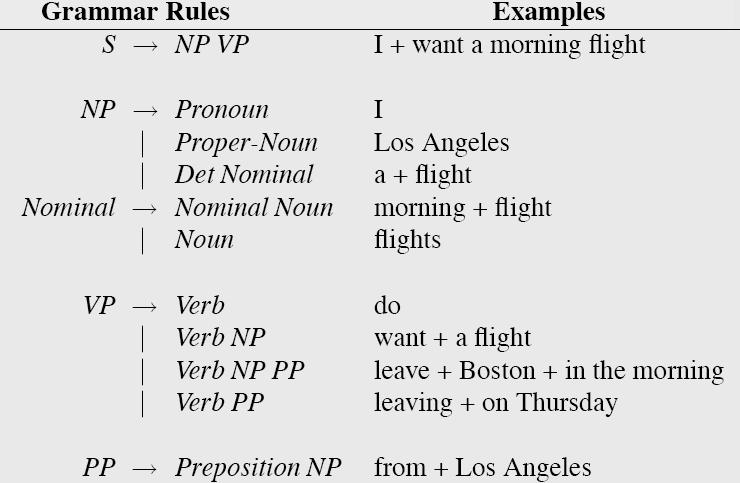
\includegraphics[scale=.4]{CFG12-3}\\
    {\large Jurafsky \& Martin 12.3}
	\end{center}
	
\end{frame}

\subsection{}
\begin{frame}{Lexicon ( Non-terminals \$rightarrow terminals )}

	\begin{description}
		\item[Noun] $\rightarrow$ flights \textpipe{} breeze \textpipe{} trip \textpipe{} morning
		\item[Verb] $\rightarrow$ is \textpipe{} prefer \textpipe{} like \textpipe{} need \textpipe{} want \textpipe{} fly
		\item[Adjective] $\rightarrow$ cheapest \textpipe{} non-stop \textpipe{} first \textpipe{} latest \textpipe{} other \textpipe{} direct
		\item[Pronoun] $\rightarrow$ me \textpipe{} I \textpipe{} you \textpipe{} it \textpipe{} they
		\item[ProperNoun] $\rightarrow$ Alaska \textpipe{} Baltimore \textpipe{} Los Angeles \textpipe{} Chicago \textpipe{} Southwest \textpipe{} Morrissey
		\item[Determiner] $\rightarrow$ the \textpipe{} a \textpipe{} an \textpipe{} this \textpipe{} these \textpipe{} that
		\item[Preposition] $\rightarrow$ from \textpipe{} to \textpipe{} on \textpipe{} near \textpipe{} above \textpipe{} through
		\item[Conjunction] $\rightarrow$ and \textpipe{} but \textpipe{} or
	\end{description}
\end{frame}


\subsection{}
\begin{frame}{}
    \setbeamercovered{invisible}

{\large As with FSAs and FSTs, you can view these rules as either analysis or synthesis machines:}
\vspace{.25cm}
	\begin{enumerate}
		\item Generate (ideally all of) the strings in the language
		\item Reject (ideall all of the) strings \textbf{not} in the language
		\item Impose hierarchical structures (trees) on strings in the language
\end{enumerate}
\end{frame}

\begin{frame}{Derivations}

{\large A derivation is a sequence of rules applied to a string that accounts for that string}
\begin{itemize}
	\item Covers all the elements in the string
	\item Covers only the elements in the string
\end{itemize}

\begin{center}
\huge{ ``All grammars leak.'' (Sapir 1921)}
\end{center}

\Tree [.S [.NP [.DET all ] [.N {grammar -s} ]] [.VP [.V leak ]]]

\end{frame}

\section{English (or part of it)}

\subsection{}
\begin{frame}{For next time:}
     \begin{block}{For next time:}
          \begin{enumerate}
     	  \item Next time we'll talk about English, TreeBanks and some more about CFGs
     	  \item Keep reading chapter 12 of Jurafsky and Martin
          \end{enumerate}
     \end{block}
\end{frame}

\subsection{}
\begin{frame}{}

\begin{columns}[c] % contents are top vertically aligned
     \begin{column}[]{3.4cm} % alternative top-align that's better for graphics
              {\Huge English! }
              \vspace{.5cm}
              \begin{enumerate}
                   \item Sentences
                   \item Noun Phrases
                  	 \hspace{.75cm}(agreement)
                   \item Verb Phrases
                  	 \hspace{.75cm}(subcategorization)
              \end{enumerate}

     \end{column}
     \begin{column}[]{7cm} % alternative top-align that's better for graphics
              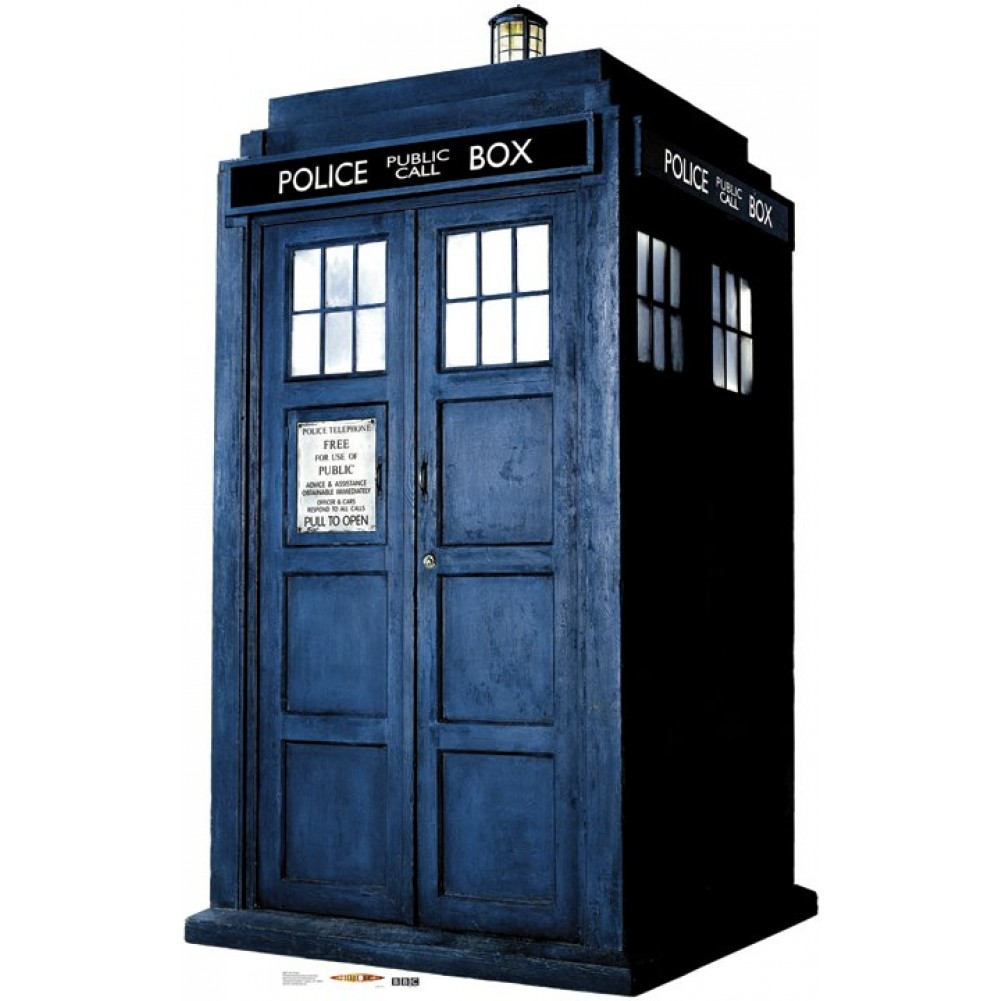
\includegraphics[scale=.3]{tardis}
     \end{column}
\end{columns}
\end{frame}

\subsection{}
\begin{frame}{Sentence Types}
\begin{description}
	\item[Declaratives] A plane left.\\
		S $\rightarrow$ NP VP
	\item[Imperatives]  Leave!\\
		S $\rightarrow$ VP
	\item[Yes-No Qs] Did the plane leave?\\
		S $\rightarrow$ Aux NP VP
	\item[WH Qs] When did the plane leave?\\
		S $\rightarrow$ WH-NP Aux NP VP
\end{description}
\end{frame}

\subsection{}
\begin{frame}{Noun Phrases}

\begin{enumerate}
	\item  NP $\rightarrow$ Det Nominal
	\item Most of the complexity of English noun phrases is hidden in this rule.
	\item Consider the derivation for the following example:
\end{enumerate}
\vspace{.5cm}
{\large All the morning flights from Denver to Tampa leaving before 10.}
\end{frame}

\subsection{}
\begin{frame}{Just one NP: [.NP [.Det All the [.Nom ... ]]}

\Tree [.Nom [.Nom [.Nom [.Nom [.Nom [.N morning ]] [.N flights ]] \qroof{from Denver}.PP ] \qroof{to Tampa}.PP ] \qroof{leaving before 10}.GerundiveVP ]

\end{frame}

\subsection{}
\begin{frame}{Noun Phrase Structure}

\begin{itemize}
	\item Clearly this NP is really about \emph{flights}. That's the central critical noun in this NP. Let
s call that the \textbf{head}.
	\item We can dissect this kind of  NP into the stuff that can come before the head, and the stuff that can come after it.
\end{itemize}
\end{frame}

\begin{frame}{Determiners}

\begin{itemize}
	\item Noun phrases can start with determiners...
	\item Determiners can be
	
	\begin{itemize}
		\item Simple lexical items: the, this, a, an, etc.\\
		A car 
		\item Or simple possessives\\
		John's car
		\item Or complex recursive versions of that\\
		John's sister's husband's son's car
	\end{itemize}
\end{itemize}
\end{frame}

\begin{frame}{Nominal}

\begin{itemize}
	\item Contains the head and any pre- and post- modifiers of the head.

	\begin{itemize}
		\item Quantifiers, cardinals, ordinals...\\
		Three cars
		\item Adjectives and APs\\
		large cars
		\item Ordering constraints\\
		Three large cars\\
		?large three cars
	\end{itemize}
\end{itemize}
\end{frame}

\begin{frame}{Post Modifiers}

	\begin{itemize}
		\item Three kinds:

		\begin{enumerate}
			\item Prepositional phrases\\
			From Seattle
			\item Non-finite clauses\\
			Arriving before noon
			\item Relative clauses\\
			That serve breakfast
		\end{enumerate}
		\item Same general (recursive) rule to handle these:\\
		\vspace{.5cm}
			Nominal $\rightarrow$ Nominal PP\\
			Nominal $\rightarrow$ Nominal GerundiveVP\\
			Nominal $\rightarrow$ Nominal RelClause\\
	\end{itemize}
\end{frame}

\begin{frame}{Agreement}

	\begin{itemize}
		\item Constraints that hold among various constituents that take part in a rule or set of rules
		\item For example, in English, determiners and the head nouns in NPs have to agree in their number.
	\end{itemize}

\begin{center}
\begin{tabular}{ l l } \toprule
    Sg N head & Pl N head \\ \midrule
    A flight & *A flights \\
	This koala & *This koalas  \\
	*Those banana & those bananas \\
	*Five cow & Five cows\\
	\bottomrule
\end{tabular}
\end{center}

\end{frame}

\begin{frame}{Problem}

	\begin{itemize}
		\item Our earlier NP rules are clearly deficient -- they don't capture this constraint!\\
NP $\rightarrow$ Det Nominal\\
	\item Accepts, and assigns correct structures to, grammatical examples (this flight)
	\item But it's also happy with incorrect examples (*these flight)
	\item Such a rule is said to \textbf{overgenerate}.

	\end{itemize}
\end{frame}

\begin{frame}{Verb Phrases}
English VPs consist of a head verb along with 0 or more following constituents which we'll call arguments.
\vspace{.5cm}
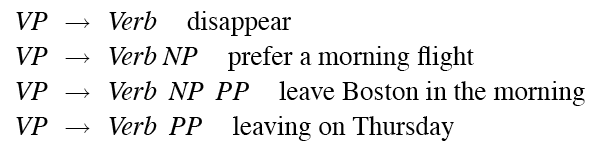
\includegraphics[scale=.4]{CFG-VP}
\end{frame}

\begin{frame}{Subcategorization}
But, even though there are many valid VP rules in English, not all verbs are allowed to participate in all those VP rules.\\
We can \textbf{subcategorize} the verbs in a language according to the sets of VP rules that they participate in.\\
This is a modern take on the traditional notion of transitive/intransitive.
Modern grammars may have 100s of such classes.
\end{frame}

\begin{frame}{Subcategorization}
\begin{description}
	\item[Sneeze]  John sneezed
	\item[Find]  Please find [a flight to NY]NP
	\item[Give] Give [me]NP[a cheaper fare]NP
	\item[Help] Can you help [me]NP[with a flight]PP
	\item[Prefer] I prefer [to leave earlier]TO-VP
	\item[Told] I was told [United has a flight]S
	\item[...]
\end{description}
\end{frame}

\begin{frame}{Subcategorization}
\begin{itemize}
	\item *John sneezed the book
	\item *I prefer United has a flight
	\item *Give with a flight
\end{itemize}

As with agreement phenomena, we need a way to formally express the constraints.
\end{frame}

\begin{frame}{Overgeneration}

Right now, our various rules for VPs overgenerate.\\

They permit the presence of strings containing verbs and arguments that don't go together.\\
\vspace{.5cm}
For example:\\

\begin{quote}
	VP $\rightarrow$ V NP
\end{quote}

	therefore Sneezed the book is a VP since `sneeze' is a verb and `the book' is a valid NP
\end{frame}

\begin{frame}{Possible CFG Solution}
\begin{columns}[c] % contents are top vertically aligned
     \begin{column}[]{5.0cm} % alternative top-align that's better for graphics
		Possible solution for agreement.\\
		\vspace{.5cm}
		Can use the same trick for all the verb/VP classes.
     \end{column}
     \begin{column}[]{5cm} % alternative top-align that's better for graphics
		SgS $\rightarrow$ SgNP SgVP\\
		PlS $\rightarrow$ PlNp PlVP\\
		SgNP $\rightarrow$ SgDet SgNom\\
		PlNP $\rightarrow$ PlDet PlNom\\
		PlVP $\rightarrow$ PlV NP\\
		SgVP $\rightarrow$ SgV Np\\
		...
     \end{column}
\end{columns}
\end{frame}

\begin{frame}{Possible CFG Solution}
\begin{enumerate}
	\item It works and stays within the power of CFGs
	\item But it's ugly
	\item And it doesn't scale all that well because of the interaction among the various constraints --explodes the number of rules in our grammar!
\end{enumerate}
\end{frame}

\begin{frame}{The Takeaway Message}

\begin{itemize}
	\item CFGs appear to be \emph{just about} what we need to account for a lot of basic syntactic structure in English.
	\item But there are problems
	\item These can be dealt with adequately, albeit inelegantly, within the CFG framework.
There are simpler, more elegant, solutions that take us out of the CFG framework (beyond its formal power)
	\item LFG, HPSG, Construction grammar, XTAG, etc.
\end{itemize}
\end{frame}

\section{Treebanks}

\begin{frame}{Treebanks}

Treebanks are corpora in which each sentence
has been paired with a parse tree (presumably
the right one).

\begin{itemize}
	\item These are generally created by first:
	\item parsing the collection with an automatic
parser
	\item And then having human annotators correct each
parse as necessary.
	\item This generally requires detailed annotation
guidelines that provide a POS tagset, a grammar
and instructions for how to deal with particular
grammatical constructions.
\end{itemize}

\end{frame}

\section{Treebanks}

\begin{frame}{Treebanks}

Treebanks implicitly define a grammar for
the language covered in the treebank.
\vspace{0.5cm}

\begin{itemize}
	\item Simply take the local rules that make up
the sub-trees in all the trees in the
collection and you have a grammar.
	\item Not complete, but if you have decent size
corpus, you'll have a grammar with decent
coverage.
	
\end{itemize}
\end{frame}

\begin{frame}{Treebank Uses}

\begin{itemize}
\item Treebanks are particularly critical to the development of
statistical parsers.
	\item The Penn Treebank's Wall Street Journal section (1,000,000 words from 1987 - 1989) is often the gold standard in statistical parsing.
\item Also valuable to Corpus Linguistics.  Investigating the empirical details of various
constructions in a given language
\end{itemize}
\end{frame}

\subsection{}
\begin{frame}{For next time:}
     \begin{block}{For next time:}
          \begin{enumerate}
     	  \item Next time we'll start statistical parsing.
     	  \item Start reading chapter 13 of Jurafsky and Martin
     	  \item Check out the new version of the syllabus!
          \end{enumerate}
     \end{block}
\end{frame}



\end{document}


